\title{Getting started with the E. Coli Whole Cell Model on Sherlock: A Brief Tutorial}


\documentclass[12pt]{article}

\usepackage{graphicx}
\usepackage[parfill]{parskip}
\usepackage{listings}
\usepackage{color}
\usepackage{underscore}

\definecolor{dkgreen}{rgb}{0,0.6,0}
\definecolor{gray}{rgb}{0.5,0.5,0.5}
\definecolor{mauve}{rgb}{0.58,0,0.82}

\lstset{frame=tb,
  language=Python,
  aboveskip=3mm,
  belowskip=3mm,
  showstringspaces=false,
  columns=flexible,
  basicstyle={\small\ttfamily},
  numbers=none,
  numberstyle=\tiny\color{gray},
  keywordstyle=\color{blue},
  commentstyle=\color{dkgreen},
  stringstyle=\color{mauve},
  breaklines=true,
  breakatwhitespace=true,
  tabsize=3
}

\begin{document}
\maketitle

\section{Basics}

This document is an introduction to running the whole-cell \textit{E. coli} model on the Sherlock computing cluster. In addition to guiding setup and providing a tutorial on modifying the model, it includes a brief primer on whole-cell model fitting in later sections.
\par
First a basic note on file locations. The knowledge base and the code that fits the knowledge base is located in the \texttt{wcEcoli/reconstruction/ecoli/} directory. The input information files are in \texttt{wcEcoli/reconstruction/ecoli/ \allowbreak flat}, and the code that loads it into an object is in \texttt{knowledge\_base\_ \allowbreak raw.py}.
\par

Processes are located in \texttt{wcEcoli/models/ecoli/processes/}. Each process represents one part of the cell's function, and they are modeled separately in short time steps and then the results of each time step are integrated between modules before initiating the next time step. RNA polymerase elongation is the process used below as an example. Other processes include translation elongation, transciption initiation, and metabolism.
\par
Each process has three components: initialize (called only once at the beginning of a simulation), calculateRequest (called at the beginning of each timestep), and evolveState (called after resources are allocated at each timestep).
\par
\emph{In initialize}: get needed parameters from the knowledge base, get views of bulk and unique molecules (bulk molecules are “indistinguishable” from each other, e.g. inactive RNAP molecules, unique molecules can be distinguished from each other, e.g. active RNAP molecules are each assigned to a location on the genome), create a view so that you can get counts, change counts, and change properties.
\par
\emph{In calculateRequest}: request the resources that you want for that timestep (don`t request all unless you are certain that another process doesn`t need this resource as well, don`t forget about metabolism).
\par
\emph{In evolveState}: perform the process, update counts, and update masses (mass must be conserved between steps).
\par
If you want to save new values to be analyzed at the end of the simulation, you must write this information out as a listener. Listeners are programs which record information during the simulation. To add a listener, add the file to \texttt{wcEcoli/models/ecoli/listeners/}, and both add an import statement and add the listener to \texttt{\_listenerClasses} in \texttt{wcEcoli/models/ecoli/sim/ \allowbreak simulation.py}.
\par
To change the cell's initial conditions, change \texttt{wcEcoli/models/ecoli/sim/ \allowbreak initial\_conditions.py}.
\par

\section{Setup}
\label{sec:setup}

This tutorial assumes you have setup access to the Sherlock cluster. If necessary before following the proceeding steps, do the following setup:

\begin{enumerate}
\item Email the research computing staff at research-computing-support@stanford.edu, and cc Professor Covert. Request access to the Sherlock cluster, and ask Professor Covert to confirm your request in the email.

\item Follow the setup instructions for logging in to Sherlock on
\linebreak
http://covert.stanford.edu/computational\_resources/sherlock/home/.

\item Follow all setup instructions in the wcEcoli/README.md file (also on the web at https://github.com/CovertLab/wcEcoli/blob/master/README.md). In particular, make sure you run
\lstset{language=bash}
\begin{lstlisting}
cd $HOME/wcEcoli
pyenv local wcEcoli
module load wcEcoli
make compile
\end{lstlisting}
\end{enumerate}

Once done with setup and these basic tutorials on Sherlock and the cluster, return to here to complete the example.



\section{Example: varying trascription rate}

\subsection{Background}

Genes encoding for stable RNA are transcribed at a faster rate in \textit{E. coli}. In the model (prior to this tutorial), all genes were transcribed at the same rate of 39~nt/s. In this tutorial, we will change the model so that genes for rRNA and tRNA are transcribed at 78~nt/s while everything else is still transcribed at 39~nt/s. 
\par

Before we start, make sure to complete the setup section (\ref{sec:setup}) if you haven't already. To begin, log in to a sherlock node. Replace 'username' with your username in the command below:

\lstset{language=bash}
\begin{lstlisting}
ssh username@sherlock
\end{lstlisting}

The code has inevitably evolved since I wrote this tutorial, so let's get on the same page by going back to an older version of the code. Let's do this tutorial on a new branch. cd into your wcEcoli directory and type the following (you only need to type enough characters of the commit checksum for it to be unique so about 10):

\lstset{language=bash}
\begin{lstlisting}
git checkout -b tutorialYourName c7b13cb809637732f993c387ae1c4b11653efdc7
\end{lstlisting}

This gives you your own copy of the specified commit of the master branch named \texttt{tutorialYourName} which you can commit to.

We need to make sure the output from the model goes to the SCRATCH filesystem (which is larger) rather than SHERLOCK\_HOME. We'll need to make a symbolic link between the output directory of your \texttt{wcEcoli} directory and a directory in SCRATCH. Within your wcEcoli diretory, there should be a folder named \texttt{out/}. The model puts its output in this folder, so we can basically tell the computer to send anything placed in this folder to SCRATCH instead.

First go to SCRATCH and create a folder in which to place the output. Run the following command:

\lstset{language=bash}
\begin{lstlisting}
cd $SCRATCH
\end{lstlisting}

Now make a directory to hold the output. You can call it whatever you want, here is one option:

\lstset{language=bash}
\begin{lstlisting}
mkdir wcEcoli_out
\end{lstlisting}

Return to your \texttt{wcEcoli} directory:

\lstset{language=bash}
\begin{lstlisting}
cd $HOME/wcEcoli
\end{lstlisting}

To create the symbolic link, we first need to delete the existing \texttt{out/} directory if it is present. Do this with:

\lstset{language=bash}
\begin{lstlisting}
rmdir out/
\end{lstlisting}

If there is no \texttt{out/} directory, then running the rmdir command won't hurt but isn't necessary. Now run this command to make the symbolic link. Change the name of the directory to the one you made on SCRATCH if it's different.

\lstset{language=bash}
\begin{lstlisting}
ln -s $SCRATCH/wcEcoli_out out
\end{lstlisting}

\subsection{Running simulations}

Now let's try running the unmodified model to make sure it works. First, log in to a compute node, so that the simulation can be run in interactive mode (running in interactive mode on a login node can result in getting booted from the cluster). These nodes are covert-lab specific and it's ok to do more serious computation on them.

\begin{lstlisting}
srun -p mcovert --ntasks-per-node=1 --time=12:00:00 --pty bash
\end{lstlisting}

It is best to run \texttt{srun} from your home directory and then \texttt{cd} into \texttt{wcEcoli} once you are on a compute node. This will load the python virtual environment nicely, which is not necessarily the case if you run \texttt{srun} from \texttt{wcEcoli} on the login node. Once you are in a compute node, ensure you are in your \texttt{wcEcoli} directory.

\begin{lstlisting}
cd $HOME/wcEcoli
\end{lstlisting}

Once you are logged into the compute node with the python virtual environment loaded, you will see the virtual environment first and the computer number next to your shell cursor like this:

\lstset{language=bash}
\begin{lstlisting}
(wcEcoli)[sunetid@sh-8-30:~/wcEcoli]$
\end{lstlisting}

Now prepare the fireworks queue with your simulation task:

\begin{lstlisting}
DESC="Tutorial run, starting code with unmodified parameters." python runscripts/fw_queue.py
\end{lstlisting}

Now the simulation task is queued up in fireworks and can be launched via:

\begin{lstlisting}
rlaunch rapidfire
\end{lstlisting}

After about a minute, this should start producing output looking something like this:

\begin{lstlisting}
(wcEcoli)[sunetidt@sh-8-30 ~/wcEcoli]$ rlaunch rapidfire
2016-04-08 14:15:30,917 INFO Hostname/IP lookup (this will take a few seconds)
2016-04-08 14:15:32,545 INFO Created new dir /home/thorst/wcEcoli/launcher_2016-04-08-21-15-32-542398
2016-04-08 14:15:32,549 INFO Launching Rocket
2016-04-08 14:15:38,572 INFO RUNNING fw_id: 17 in directory: /home/thorst/wcEcoli/launcher_2016-04-08-21-15-32-542398
2016-04-08 14:15:38,577 INFO Task started: {{wholecell.fireworks.firetasks.initRawData.InitRawDataTask}}.
Fri Apr  8 14:15:38 2016: Instantiating raw_data
Fri Apr  8 14:15:43 2016: Saving raw_data
2016-04-08 14:15:43,868 INFO Task completed: {{wholecell.fireworks.firetasks.initRawData.InitRawDataTask}} 
2016-04-08 14:15:50,912 INFO Rocket finished
2016-04-08 14:15:51,258 INFO Created new dir /home/thorst/wcEcoli/launcher_2016-04-08-21-15-51-256566
2016-04-08 14:15:51,261 INFO Launching Rocket
2016-04-08 14:15:54,788 INFO RUNNING fw_id: 15 in directory: /home/thorst/wcEcoli/launcher_2016-04-08-21-15-51-256566
2016-04-08 14:15:54,791 INFO Task started: {{wholecell.fireworks.firetasks.fitSimData.FitSimDataTask}}.
Fri Apr  8 14:15:54 2016: Creating/Fitting sim_data (Level 1)
 \end{lstlisting}

\hfill \break

Then once the actual simulation starts, you will see:

\hfill \break

\begin{lstlisting}
Fri Apr  8 14:19:50 2016: Running simulation
Time (s)  Dry mass     Dry mass      Protein          RNA     Expected
              (fg)  fold change  fold change  fold change  fold change
========  ========  ===========  ===========  ===========  ===========
       0    245.46        1.000        1.000        1.000        1.000
       0    245.49        1.000        1.000        1.000        1.000
       0    245.52        1.000        1.000        1.000        1.000
       0    245.54        1.000        1.000        1.000        1.000
       0    245.56        1.000        1.000        1.000        1.000
       1    245.65        1.001        1.000        1.000        1.000
       1    245.74        1.001        1.000        1.000        1.000
       2    245.82        1.001        1.001        1.000        1.001
       3    245.90        1.002        1.001        1.000        1.001
       4    245.98        1.002        1.001        1.000        1.001
       5    246.05        1.002        1.001        0.999        1.001
       6    246.12        1.003        1.001        0.999        1.001
       7    246.18        1.003        1.002        0.999        1.001
       8    246.24        1.003        1.002        0.999        1.002
       9    246.30        1.003        1.002        0.999        1.002
       9    246.37        1.004        1.002        0.999        1.002
      10    246.43        1.004        1.002        0.999        1.002
      11    246.49        1.004        1.002        1.000        1.002
      12    246.55        1.004        1.003        1.000        1.002
      13    246.62        1.005        1.003        1.000        1.003
      14    246.68        1.005        1.003        1.000        1.003
      15    246.74        1.005        1.003        1.000        1.003
      16    246.80        1.005        1.003        1.000        1.003
      17    246.87        1.006        1.004        1.000        1.003
      17    246.93        1.006        1.004        1.000        1.003
      18    246.98        1.006        1.004        1.000        1.004
      19    247.03        1.006        1.004        1.000        1.004
      20    247.07        1.007        1.004        1.000        1.004
      21    247.12        1.007        1.004        1.000        1.004
      22    247.16        1.007        1.005        1.000        1.004
      23    247.21        1.007        1.005        1.001        1.005
      24    247.25        1.007        1.005        1.001        1.005
      25    247.30        1.007        1.005        1.001        1.005
      26    247.34        1.008        1.005        1.001        1.005
      26    247.38        1.008        1.005        1.001        1.005
      27    247.43        1.008        1.006        1.001        1.005
      28    247.47        1.008        1.006        1.001        1.006
      29    247.52        1.008        1.006        1.001        1.006
      30    247.56        1.009        1.006        1.001        1.006
      31    247.60        1.009        1.006        1.002        1.006
      32    247.65        1.009        1.007        1.002        1.006
      33    247.69        1.009        1.007        1.002        1.006
      34    247.73        1.009        1.007        1.002        1.007
      34    247.78        1.009        1.007        1.002        1.007
      35    247.82        1.010        1.007        1.002        1.007
      36    247.86        1.010        1.007        1.002        1.007
      37    247.91        1.010        1.008        1.002        1.007
      38    247.95        1.010        1.008        1.003        1.007
      39    248.00        1.010        1.008        1.003        1.008
      40    248.04        1.011        1.008        1.003        1.008
\end{lstlisting}

\hfill \break
\hfill \break

This will take a few minutes to run. At the end you can find the output in the \texttt{out/timestamp} directory (timestamp obviously replaced with the actual timestamp of when you started the simulation). Look at the plots in the \texttt{/wcEcoli/out/20150623.190922.827654/wildtype\_000000/000000/ \allowbreak generation\_000000/000000/plotOut} directory (replacing the timestamp directory with your own timestamped directory name).


\subsection{Add a new parameter to the model}

First, let's add a new elongation rate to the knowledge base. In \texttt{reconstruction/ \allowbreak ecoli/flat} is a tsv called \texttt{growthRateDependentParameters.tsv}. Add a new column for the fast rna polymerase rate (estimate that it is double the normal rate). The normal rate at each growth rate is stored in the column ``rnaPolymeraseElongationRate''. This command will generate the file with the new column appended, or edit the file in a different way if desired.

\begin{lstlisting}
awk '{if(NR==1){print $0 "\t" "rnaPolymeraseElongationRateFast (units.nt/units.s)"}else{print $0 "\t" ($9*2)}}' growthRateDependentParameters.tsv > temp && mv temp growthRateDependentParameters.tsv  
\end{lstlisting}

Alternatively, you could open the .tsv file in a spreadsheet editor and add the new column by hand.

To check that the parameter was added, examine the knowledge base object in ipython after switching back to the \texttt{wcEcoli} directory.

\lstset{language=Python}
\begin{lstlisting}
ipython
import reconstruction.ecoli.knowledge_base_raw as kbr
kb=kbr.KnowledgeBaseEcoli()
kb.growthRateDependentParameters[0]
\end{lstlisting}

You should see the \texttt{'rnaPolymeraseElongationRateFast': 78 [nucleotide/s]} entry in the resulting dictionary.

\subsection{Create a new process}

Let's split the transcript elongation process into a slow process and a fast process. Go to \texttt{models/ecoli/processes/} :

\lstset{language=bash}
\begin{lstlisting}
cd models/ecoli/processes/

cp transcript_elongation.py transcript_elongation_fast.py

mv transcript_elongation.py transcript_elongation_slow.py
\end{lstlisting}

Now we need to add these processes to the simulation, so that they actually get called. Let's go back to the \texttt{wcEcoli} directory. Open \texttt{models/ecoli/sim/ \allowbreak simulation.py} and change line 17 to read: 

\lstset{language=Python}
\begin{lstlisting}
from models.ecoli.processes.transcript_elongation_slow import TranscriptElongationSlow
\end{lstlisting}

Then add a line just under this:

\begin{lstlisting}
from models.ecoli.processes.transcript_elongation_fast import TranscriptElongationFast
\end{lstlisting}

Under process classes, add \texttt{TranscriptElongationFast} and change \texttt{Transcript \allowbreak Elongation} to \texttt{TranscriptElongationSlow}. \texttt{\_processClasses} should now look like this:


\begin{lstlisting}
        _processClasses = (
                Metabolism,
                RnaDegradation,
                TranscriptInitiation,
                TranscriptElongationSlow,
                TranscriptElongationFast,
                PolypeptideInitiation,
                PolypeptideElongation,
                ReplicationElongation,
                ProteinDegradation,
                Complexation,
                ChromosomeFormation,
                Equilibrium,
                )
\end{lstlisting}

\subsection{Change the model output}

Now let's change the listeners to record output from these new processes. We write data to listeners, and the listener is responsible for recording the data to the file, as well as transforming it as necessary (calculating averages, for example). The transcription submodels write to three listeners: \texttt{GrowthLimits}, \texttt{RnapData}, and \texttt{TranscriptElongationListener}. We need to make several changes in order to correctly log transcription data. The fast and slow transcription submodels need to both write to the same listener attributes, so we need to set them up to add data together, rather than overwriting one another's output.

First, we need to update the listeners to zero out the relevant attributes each time step, so that we can add to them from each model. Open \texttt{models/ \allowbreak ecoli/listeners/growth\_limits.py} and add the following lines to the end of \texttt{tableAppend(...)}, after line 99:

\lstset{language=Python}
\begin{lstlisting}
self.ntpRequestSize = np.zeros(len(self.ntpIds), np.float64)
self.ntpAllocated = np.zeros(len(self.ntpIds), np.float64)
self.ntpUsed = np.zeros(len(self.ntpIds), np.float64)
\end{lstlisting}

We need to make two changes to \texttt{models/ecoli/listeners/rnap\_data.py}. At line 73, update the lines that read:
\lstset{language=Python}
\begin{lstlisting}
self.ntpCountInSequence = np.zeros(21, np.int64)
self.ntpCounts = np.zeros(21, np.int64)
\end{lstlisting}

To read:
\lstset{language=Python}
\begin{lstlisting}
self.ntpCountInSequence = np.zeros(0, np.int64)
self.ntpCounts = np.zeros(0, np.int64)
\end{lstlisting}

This initializes some arrays we'll be writing to to be completely empty, which allows us to append to them without having a bunch of leading data we don't want. Next, we reset the relevant attributes as in \texttt{GrowthLimits}. Add the following to the bottom of \texttt{tableAppend(...)}, after line 117:
\lstset{language=Python}
\begin{lstlisting}
self.rnapStalls = np.zeros(0, np.int64)
self.ntpCountInSequence = np.zeros(0, np.int64)
self.ntpCounts = np.zeros(0, np.int64)
self.expectedElongations = 0
self.actualElongations = 0
self.didTerminate = 0
self.terminationLoss = 0
\end{lstlisting}

Finally, we need to update \texttt{models/ecoli/listeners/transcript\_elongation \allowbreak \_listener.py}. Add to the bottom of \texttt{tableAppend(...)}, after line 43:
\lstset{language=Python}
\begin{lstlisting}
self.countRnaSynthesized = np.zeros(self.countRnaSynthesized.shape, self.countRnaSynthesized.dtype)
\end{lstlisting}

\subsection{Modify a process}

Now let's modify the new processes. Open \texttt{models/ecoli/processes/transcript \allowbreak \_elongation\_slow.py} and change all references of \texttt{TranscriptElongation} to \texttt{TranscriptElongationSlow}.

Next create a Boolean vector that is True at the indices of transcripts that should be elongated at the slow rate and False at the indices of transcripts that should be elongated at the fast rate. In the initialize function add the following line (after line 73):

\lstset{language=Python}
\begin{lstlisting}
self.slowRnaBool = ~(sim_data.process.transcription.rnaData["isRRna5S"] | sim_data.process.transcription.rnaData["isRRna16S"] | sim_data.process.transcription.rnaData["isRRna23S"] | sim_data.process.transcription.rnaData["isTRna"])
\end{lstlisting}

\texttt{isRRna5S}, \texttt{isRRna16S}, \texttt{isRRna23S}, and \texttt{isTRna} are properties of \texttt{rnaData}, which is found in the simulation data set (\texttt{sim\_data}). These are vectors of Boolean values. The tilde inverts the boolean value, so this creates a vector that is False for all 5S rRNA, 16S rRNA, 23S rRNA, and tRNA, and True for everything else.
Now let's change the view onto the active RNA polymerases to a view onto only the active RNA polymerases that are on transcripts that should be elongated at the slow rate. Change the definition of \texttt{self.activeRnaPolys} (line 79) to read:

\begin{lstlisting}
self.activeRnaPolys = self.uniqueMoleculesView('activeRnaPoly',
	rnaIndex = ("in", np.where(self.slowRnaBool)[0]))
\end{lstlisting}

Next, we need to update our writes to the listeners to increment or append, rather than overwrite, the attributes that are updated. First, add a new import at the top of the file (after line 25):
\begin{lstlisting}
from wholecell.listeners.listener import WriteMethod
\end{lstlisting}

Second, we need to change our calls to \texttt{writeToListener(...)} to either increment (in the case of numeric attributes), or append (in the case of arrays), rather than overwriting. Modify all of the \texttt{writeToListener(...)} calls (except for \texttt{ntpPoolSize}) since this is one value that both slow and fast elongation see, to have a new parameter at the end:  \texttt{WriteMethod.increment}, except for the writes to \texttt{rnapStalls}, \texttt{ntpCountInSequence}, and \texttt{ntpCounts}, which instead should have \texttt{WriteMethod.append}. Overall, the lines should look like the following (although in the file they are scattered around a bit):

\begin{lstlisting}
self.writeToListener("GrowthLimits", "ntpRequestSize", maxFractionalReactionLimit * sequenceComposition, WriteMethod.increment)

self.writeToListener("GrowthLimits", "ntpAllocated", self.ntps.counts(), WriteMethod.increment)

self.writeToListener("TranscriptElongationListener", "countRnaSynthesized", terminatedRnas, WriteMethod.increment)

self.writeToListener("GrowthLimits", "ntpUsed", ntpsUsed, WriteMethod.increment)
self.writeToListener("RnapData", "rnapStalls", rnapStalls, WriteMethod.append)
self.writeToListener("RnapData", "ntpCountInSequence", ntpCountInSequence, WriteMethod.append)
self.writeToListener("RnapData", "ntpCounts", ntpCounts, WriteMethod.append)
self.writeToListener("RnapData", "expectedElongations", expectedElongations.sum(), WriteMethod.increment)
self.writeToListener("RnapData", "actualElongations", sequenceElongations.sum(), WriteMethod.increment)
self.writeToListener("RnapData", "didTerminate", didTerminate.sum(), WriteMethod.increment)
self.writeToListener("RnapData", "terminationLoss", (terminalLengths - transcriptLengths)[didTerminate].sum(), WriteMethod.increment)
\end{lstlisting}

This is all we need to change in this file. Now let's open the fast transcript elongation file \texttt{models/ecoli/processes/transcript\_elongation \allowbreak \_fast.py}. Similarly to what we did in the slow elongation file, let's change all references of \texttt{TranscriptElongation} to \texttt{TranscriptElongationFast}.

Next, let's change the elongation rate. Change line 60 to read:

\begin{lstlisting}
self.rnapElngRate = sim_data.growthRateParameters.rnaPolymeraseElongationRateFast.
	 asNumber(units.nt / units.s)
\end{lstlisting}

Now, let's create the opposite of the Boolean vector that we created in \texttt{transcript\_elongation\_slow.py}. In the initialize function add the following line (after line 74):

\lstset{language=Python}
\begin{lstlisting}
self.fastRnaBool = (sim_data.process.transcription.rnaData["isRRna5S"] | sim_data.process.transcription.rnaData["isRRna16S"] | sim_data.process.transcription.rnaData["isRRna23S"] | sim_data.process.transcription.rnaData["isTRna"])
\end{lstlisting}

Now let's change the view onto the active rna polymerases to a view onto only the active RNA polymerases that are on transcripts that should be elongated at the fast rate (line 80):

\begin{lstlisting}
self.activeRnaPolys = self.uniqueMoleculesView('activeRnaPoly',
	rnaIndex = ("in", np.where(self.fastRnaBool)[0]))
\end{lstlisting}

Also, we need to update our writes to the listeners as before. First, add a new import at the top of the file (after line 25):
\begin{lstlisting}
from wholecell.listeners.listener import WriteMethod
\end{lstlisting}

Finally, update the \texttt{writeToListener(...)} lines to match the changes you made in \texttt{TranscriptElongationSlow}, above. Now data from both submodels will be recorded in the whole cell output.

Now let's change the calculation of the RNA polymerase activation rate. In the model, an RNA polymerase can either be active or inactive:

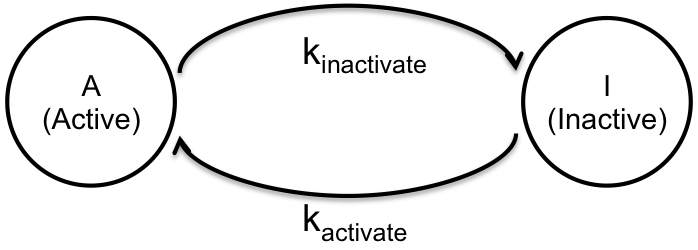
\includegraphics{img.png}


To calculate the rate of activation, $k_{activate}$, we write an equation for the rate of change of the number of RNAP active at steady state:

$$
\frac{dA}{dt}=k_{activate}I - k_{inactivate}A=0
$$

This gives us that

$$
k_{activate} = k_{inactivate}\frac{A}{I}
$$


We know from experiments the fraction of RNA polymerases that are active, $f_{active}$:

$$
f_{active}=\frac{A}{A+I}
$$

Using that 

$$
f_{active} = 1 - f_{inactive}
$$

We can rearrange and solve for the rate of activation:

$$
k_{activate}=k_{inactivate}\left(\frac{f_{active}}{1-f_{active}} \right)
$$

We can calculate the rate of inactivation from the elongation rate, the transcript lengths, and the synthesis probabilities:

$$
k_{inactivate}=\frac{k_{elong}}{L_i}\cdot\frac{1}{p_{synth}}
$$

We want to change the elongation rate to be a vector, rather than a constant:

$$
k_{inactivate}=\frac{k_{elong,i}}{L_i}\cdot \frac{1}{p_{synth}}
$$

Now let's do this in the code. In \texttt{models/ecoli/processes/transcript \allowbreak \_initiation.py}, first add some lines to the initialize function so we can access data in another function.  After line 56, add the following:

\begin{lstlisting}
self.rnaPolymeraseElongationRateFast = sim_data.growthRateParameters.rnaPolymeraseElongationRateFast
\end{lstlisting}

Below this after line 69, add:

\begin{lstlisting}
self.is_tRNA = sim_data.process.transcription.rnaData['isTRna']
\end{lstlisting}

Next, add a line to pass the fast elongation rate to the function we would like to change.  On line 80, change the function call to look like the following:

\begin{lstlisting}
self.activationProb = self._calculateActivationProb(
	 self.fracActiveRnap,
	 self.rnaLengths,
	 self.rnaPolymeraseElongationRate,
	 self.rnaPolymeraseElongationRateFast,
	 self.rnaSynthProb,
	 )
\end{lstlisting}

Now, we need to make some changes to the \texttt{\_calculateActivationProb} function (on line 145). Change the function definition to the following:

\begin{lstlisting}
def _calculateActivationProb(self, fracActiveRnap, rnaLengths, rnaPolymeraseElongationRate, rnaPolymeraseElongationRateFast, synthProb):
\end{lstlisting}

The following lines should be adding at the top of the function. The tilde operator inverts the booleans.

\begin{lstlisting}
fastRnaBool = self.is_5SrRNA | self.is_16SrRNA | self.is_23SrRNA | self.is_tRNA
slowRnaBool = ~fastRnaBool
\end{lstlisting}

Now, add a line below this for a vector of the elongation rate for each RNA strand:

\begin{lstlisting}
elngRateVector = rnaPolymeraseElongationRate * slowRnaBool +  rnaPolymeraseElongationRateFast * fastRnaBool
\end{lstlisting}

Now change the next line to reflect the new rate vector:

\begin{lstlisting}
expectedTranscriptionTime = 1. / elngRateVector * rnaLengths
\end{lstlisting}

\par
Now we can run a simulation and rRNA and tRNA would be transcribed at the new fast rate, while everything else was transcribed at the same slow rate before. Follow these steps to run the new simulation code:
\par
Queue up the tasks in fireworks:

\lstset{language=bash}
\begin{lstlisting}
DESC="Tutorial run, adding different RNA polymerization rate for r- and t- RNAs." python runscripts/fw_queue.py
\end{lstlisting}

Run the tasks in the queue until finished:

\begin{lstlisting}
rlaunch rapidfire
\end{lstlisting}

To check for the success of your simulation, open the \texttt{wcEcoli/out/} folder, and the folder timestamped to the simulation just run, then click through to the output plots. Specifically, look at the \texttt{massFractionSummary} plot. Does everything roughly double in one cell cycle? If not, why might that be?

\subsection{Changing the fitting}

Even though we've changed the model, the simulation will be initialized the same way as before. This is a problem because before running a simulation, we need to fit several parameters such as the initial counts of RNA polymerases. Because some things are now being transcribed at a faster rate, we should need fewer RNA polymerases to make the same number of transcripts. Additionally, if some things are being transcribed more quickly, then RNA polymerases will be inactivating more quickly. In order to maintain a constant ratio of active to inactive RNA polymerases (experimentally shown to be around 20\%), the activation rate must also increase now. 

\par

We calculate the number of RNA polymerases that we need initially by writing an equation for the rate of change of some RNA $R_i$ (rate of synthesis - rate of degradation = rate of dilution due to growth):

$$
\frac{d R_i}{dt} = \frac{k_{elong}}{L_i}P_i(t) - \frac{\ln(2)}{h_i}R_i(t) = \frac{\ln(2)}{\tau_d}R_i(t)
$$


$L_i$ is the length of transcript $i$; $P_i$ is the number of RNA polymerases actively transcribing $R_i$ at time $t$; $h_i$ is the half life of $R_i$; $\tau_d$ is the length of the cell cycle; $k_{elong}$ is the transcript elongation rate. Right now this is a constant value for all transcripts. We want to change this to be different for rRNA and tRNA. Let's change this in the code. Open the file \texttt{reconstruction/ecoli/fit\_sim\_data\_1.py} and go to the \texttt{setRNAPCounts \allowbreak ConstrainedByPhysiology} function. This is what we need to change. Let's add the Boolean vectors for fast and slow transcripts. Right at the beginning of this function definition (after line 473), add these two lines:

\lstset{language=Python}
\begin{lstlisting}
fastRnaBool = (sim_data.process.transcription.rnaData["isRRna5S"] | sim_data.process.transcription.rnaData["isRRna16S"] | sim_data.process.transcription.rnaData["isRRna23S"] | sim_data.process.transcription.rnaData["isTRna"])
slowRnaBool = ~fastRnaBool
\end{lstlisting}

Let's break up the calculation of \texttt{nActiveRnapNeeded} into \texttt{nActiveRnapNeeded \allowbreak ForFast} and \texttt{nActiveRnapNeededForSlow}. Change the \texttt{nActiveRnapNeeded} calculation on line 507 to read:

\begin{lstlisting}
nActiveRnapNeededForSlow = calculateMinPolymerizingEnzymeByProductDistributionRNA(
    rnaLengths[slowRnaBool], 
    sim_data.growthRateParameters.rnaPolymeraseElongationRate, 
    rnaLossRate[slowRnaBool])
\end{lstlisting}

Add a line under this for the calculation for the fast transcripts:

\begin{lstlisting}
nActiveRnapNeededFast = calculateMinPolymerizingEnzymeByProductDistributionRNA(
    rnaLengths[fastRnaBool], 
    sim_data.growthRateParameters.rnaPolymeraseElongationRateFast, 
    rnaLossRate[fastRnaBool])
\end{lstlisting}

Below this, add a line to calculate the total number of RNA polymerases needed:

\begin{lstlisting}
nActiveRnapNeeded = nActiveRnapNeededForFast + nActiveRnapNeededForSlow
\end{lstlisting}

Now the fitting of the initial number of RNA polymerases and the activation rate is fixed. We can run a simulation and the model will reflect changes to both the processes and fitting for rRNA and tRNA to be transcribed at the new fast rate. Queue up the tasks in fireworks:

\lstset{language=bash}
\begin{lstlisting}
DESC="Tutorial run, updated model fitting." python runscripts/fw_queue.py
\end{lstlisting}

Run the tasks in the queue until finished:

\begin{lstlisting}
rlaunch rapidfire
\end{lstlisting}

Check the output to make sure that the RNA mass fractions more closely double over the cell cycle.


\end{document}
